% id: 17-17
% book: 베이직쎈 확률과 통계 · 01 여러 가지 순열
% section: 유형 010 최단 거리로 가는 경우의 수; 중간 지점을 잡아야 하는 경우
% figure: none
% answer: 
% answer_source: 
% variant_level: 0 (원본 전사)
% 이 파일은 build.mjs 가 items.json 에서 만든다. 고칠 때는 items.json 을 고친다.
\smash{\raisebox{1.5mm}{\dmkichul{베이직쎈 확률과 통계 17쪽 17번}}}
다음 그림과 같은 도로망이 있다. $\pt{A}$에서 $\pt{B}$까지 최단 거리로 가는 경우의 수를 구하시오.
\dmsubprob{1} % 17-17 ⑴(본책 17쪽) — 계단 모양 도로망(왼쪽 아래 2칸×1칸 블록 + 그 오른쪽 위로 2칸×2칸 블록 · 두 블록은 가운데 가로줄로 이어진다). A 왼쪽 아래 · B 오른쪽 위. 스캔 그림을 TikZ 로 다시 그림(스캔 화질).
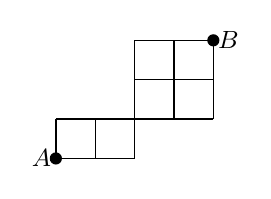
\begin{tikzpicture}[line width=0.5pt]
  % 아래 블록(가로 2칸·세로 1칸)
  \foreach \x in {0, 0.5, 1} { \draw (\x,0) -- (\x,0.5); }
  \draw (0,0) -- (1,0);
  % 두 블록을 잇는 가운데 가로줄
  \draw (0,0.5) -- (2,0.5);
  % 위 블록(가로 2칸·세로 2칸)
  \foreach \x in {1, 1.5, 2} { \draw (\x,0.5) -- (\x,1.5); }
  \foreach \y in {1, 1.5} { \draw (1,\y) -- (2,\y); }
  \fill (0,0) circle (2.2pt);
  \node[left, font=\small, inner sep=1.5pt] at (0,0) {$\pt{A}$};
  \fill (2,1.5) circle (2.2pt);
  \node[right, font=\small, inner sep=1.5pt] at (2,1.5) {$\pt{B}$};
\end{tikzpicture}

\dmsubprob{2} % 17-17 ⑵(본책 17쪽) — 가로 4칸·세로 3칸 도로망에서 가운데 가로줄 사이의 세로 도로 한 칸(왼쪽에서 둘째 세로줄·가운데 띠)이 없는 그림. A 왼쪽 위 · B 오른쪽 아래. 스캔 그림을 TikZ 로 다시 그림(스캔 화질).
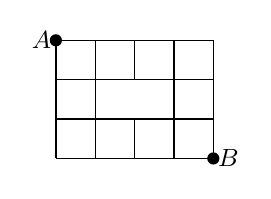
\begin{tikzpicture}[line width=0.5pt]
  \foreach \y in {0, 0.5, 1, 1.5} { \draw (0,\y) -- (2,\y); }
  \foreach \x in {0, 0.5, 1.5, 2} { \draw (\x,0) -- (\x,1.5); }
  \draw (1,0) -- (1,0.5);
  \draw (1,1) -- (1,1.5);
  \fill (0,1.5) circle (2.2pt);
  \node[left, font=\small, inner sep=1.5pt] at (0,1.5) {$\pt{A}$};
  \fill (2,0) circle (2.2pt);
  \node[right, font=\small, inner sep=1.5pt] at (2,0) {$\pt{B}$};
\end{tikzpicture}

